Para el desarrollo de este proyecto, se hizo un estudio de mercado tanto de los
consumidores como de sus características, además de una evaluación exhaustiva
de qué les gustaría tener en su vehículo.

Este proyecto pretende en un futuro salir a mercado y suplir características que los
usuarios echan en falta en sus correspondientes medios de transporte. Como en principio
funciona con cualquier vehículo que cuente con \ac{OBD}--II, las respuestas no se han
limitado a aquellos conductores que condujesen turismos sino cualquier tipo de
automóvil: motocicleta, camión, etc.

Es importante destacar que el estudio tiene varios sesgos que han restringido
y delimitado las respuestas que se han registrado:

\begin{enumerate}
  \item Se ha realizado un cuestionario usando Google Forms, una plataforma de Google
        que permite preparar una serie de preguntas y respuestas y aplicar ciertos
        filtros sobre ellas. Por ejemplo, para aquellos que dijeron ser conductores,
        se hicieron preguntas diferentes frente a quienes no lo fueran.

        Esto permite obtener datos más fidedignos y acotados según la población que
        respondiera. Sin embargo, tiene una limitación implícita: restringe el acceso
        a aquellos con conocimientos ``suficientes'' acerca de la plataforma. Pese
        a que el producto pretende ser lo más accesible posible, no hay que olvidar
        que este tipo de tecnologías permanecen desconocidas para una gran parte
        de la población con escasos conocimientos acerca de Internet o de las
        nuevas tecnologías. Se comentará más adelante, pero esto se ve reflejado
        principalmente en la edad media de quienes respondieron el cuestionario.

        Por otra parte, al ser un cuestionario aparece otra limitación implícita
        y es la validación y verificación de las respuestas: se confía en la buena
        fe de los participantes y en la calidad de sus respuestas. Igualmente, se
        desarrolló el cuestionario junto con una psicóloga que ayudó a definir
        preguntas cerradas e incluir ciertas respuestas de control. Por otra parte,
        se usó el propio mecanismo que ofrece este servicio de Google para ordenar
        aleatoriamente las respuestas del cuestionario (y que eso sirviese también
        como control).

  \item Los encuestados fueron contactados principalmente por la red social Twitter,
        mediante la difusión con ``me gusta'' y ``retweet''. También se usaron otros
        medios de comunicación (como el correo UPM y Telegram/WhatsApp), pero el
        mayoritario fue el ya mencionado. Nuevamente, esto introduce un sesgo tanto
        por edad como por accesibilidad.

  \item Junto con la encuesta, se realizó un sorteo entre aquellos que respondiesen
        a la misma de un cheque regalo de Amazon valorado en 20\EUR{}. Si bien este
        incentivo pudiera resultar interesante, puede resultar también en un nuevo
        sesgo en donde personas que o bien no compren en Amazon o bien no sepan
        lo que es no quisieran hacer el cuestionario.

        Además, se plantea la casuística en que ciertas personas quisieran responder
        al cuestionario solo por el cheque de Amazon, sin importar la calidad de
        las respuestas, ``ensuciando'' los resultados obtenidos y quitándole credibilidad
        al cuestionario en sí.

        Esto se analizará posteriormente junto con las respuestas recibidas y las
        preguntas de control introducidas.

  \item El cuestionario, al ser relativamente exhaustivo, pudo echar para atrás a muchos
        posibles encuestados ya que se estima que el tiempo medio para realizarlo es del
        orden de 10/15 minutos. A parte del daño evidente de tener menos muestra con la
        que trabajar, este posible suceso reduciría también la variedad de la población
        y la calidad del estudio realizado.
\end{enumerate}

La primera pregunta que se realizó a los encuestados era si eran conductores o no.
Los datos revelan que el $72.7\%$ ($16$) de los encuestados es conductor, mientras que el
$27.3\%$ ($6$) restante no, del total que fueron $22$ (figura \ref{fig:drivers-nodrivers}):

\begin{figure}[H]
  \centering
  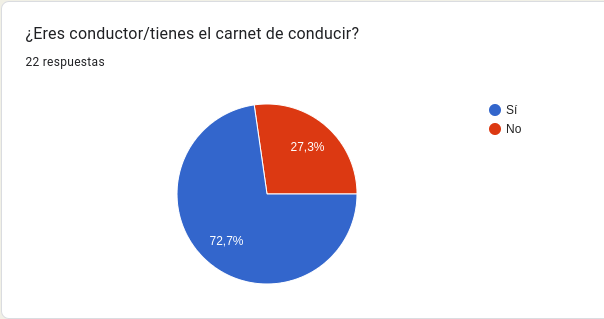
\includegraphics[width=\linewidth]{images/drivers-nodrivers.png}
  \caption{Gráfico de tarta que muestra quiénes de los encuestados son conductores ($72.7\%$) y quiénes no ($27.3\%$).}
  \label{fig:drivers-nodrivers}
\end{figure}

% Se preguntó a continuación por el tiempo de carnet que tenía cada conductor:

% \begin{figure}[H]
%   \centering
%   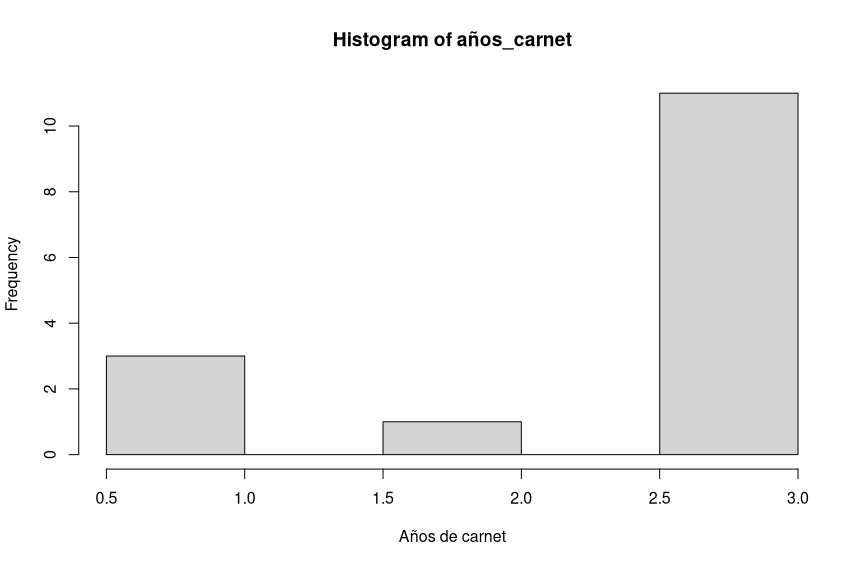
\includegraphics[width=\linewidth]{images/carnet-time.png}
%   \caption{Años de carnet.}
% \end{figure}
